\documentclass[12pt]{kiarticle}
\graphicspath{{pictures/}}
\DeclareGraphicsExtensions{.pdf,.png,.jpg,.eps}
%%%
\pagestyle{fancy}
\fancyhf{}
%\renewcommand{\headrulewidth}{ 0.1mm }
\renewcommand{\footrulewidth}{ .0em }
\fancyfoot[C]{\texttt{\textemdash~\thepage~\textemdash}}
\fancyhead[L]{Лабораторная работа № 6.11.1 \hfil}
\fancyhead[R]{\hfil Иванов Кирилл, 625 группа }
\usepackage{multirow} % Слияние строк в таблице
\newcommand
{\un}[1]
{\ensuremath{\text{#1}}}
\newcommand{\eds}{\ensuremath{ \mathscr{E}}}
\newcommand{\ga}{\ensuremath{\gamma}}
\usepackage{tikz}
%%% Работа с таблицами
\usepackage{array,tabularx,tabulary,booktabs} % Дополнительная работа с таблицами
\usepackage{longtable}  % Длинные таблицы
\usepackage{multirow} % Слияние строк в таблице

\begin{document}
	
	\begin{titlepage}
		\begin{center}
			\large 	Московский физико-технический институт \\
			(национальный исследовательский университет) \\
			Факультет общей и прикладной физики \\
			\vspace{0.2cm}
			
			\vspace{4.5cm}
			Лабораторная работа №6.11.1  \\ \vspace{0.2cm}
			\large (Основы современной физики) \\ \vspace{0.2cm}
			\LARGE \textbf{ Определение ширины запрещенной зоны полупроводника  }
		\end{center}
		\vspace{2.3cm} \large
		
		\begin{center}
			Работу выполнил: \\
			Иванов Кирилл,
			625 группа
			\vspace{10mm}		
			
		\end{center}
		
		\begin{center} \vspace{60mm}
			г. Долгопрудный \\
			2019 год
		\end{center}
	\end{titlepage}


	\paragraph*{Цель работы:} исследовать температурную зависимость проводимости полупроводника; определить ширину запрещенной зоны полупроводника из полученной зависимости.
	
	\section{Теоретическое введение }
	\subsection{Температурная зависимость проводимости металлов}
	
	Свойства металлов достаточно хорошо описываются \textit{моделью свободных электронов}: в отсутствии внешних полей электроны движутся прямолинейно и с постоянной скоростью, столкновения их друг с другом и с ионами считаются мгновенными. 
	
	При наличии постоянного электрического поля $E$ возникает постоянный ток, и дрейфовая скорость электронов равна: 
	
	\[ v_d = \frac{eE\tau}{m} \]
	
	Здесь $\tau$ - время релаксации. 
	
	Из закона Ома, плотность тока $j$ пропорциональна напряженности поля $E$: $j = \sigma E$, $\sigma$ - удельная проводимости вещества. 
	
	С учетом выражения для плотности тока $j = env_d$, где $n$ - концентрация электронов, получим: 
	
	\[ \sigma = \frac{j}{E} = \frac{ne^2\tau}{m} \]
	
	Концентрация $n$ электронов в зоне проводимости мало зависит от температуры, а время релаксации $\tau$ уменьшается при нагревании из-за увеличения числа фононов. Причем в большом диапазоне температур верно: 
	
	\[ \sigma_m \propto 1/T \]
	
	\subsection{Температурная зависимость проводимости полупроводников}
	
	Проводимость в полупроводниках зависит от количества электронов в зоне проводимости и дырок в валентной зоне. 
	
	Вероятность заполнения $f(\epsilon)$ энергетических уровней электронами определяется функцией Ферми: 
	
	\[ f(\epsilon) = \frac{1}{1 + \exp\left(\frac{\epsilon - \mu}{kT}\right)} \]
	
	Здесь $\epsilon$ - значение энергии уровня в зоне проводимости, $\mu$ - уровень Ферми. 
	
	В приближении $(\epsilon - \mu) >> kT$ имеем: 
	
	\[ f(\epsilon) \approx \exp\left(-\frac{\epsilon - \mu}{kT}\right) \] 
	
	При небольших температурах электроны занимают нижние уровни, то есть $\epsilon \approx \epsilon_c$, $\epsilon_c$ - энергия, соответствующая дну зоны проводимости. Тогда количество электронов $n_n$ равно: 
	
	\[ n_n = Q_n\cdot f(\epsilon) \approx Q_n\exp\left(-\frac{\epsilon_c - \mu}{kT}\right) \]
	
	Здесь $Q_n$ - количество занятых электронами уровней.
	
	Вероятность возникновения дырки равна $1 - f(\epsilon)$. В рассматриваемом приближении энергию дырок будем считать равной энергии верхней границы валентной зоны $\epsilon_v$, тогда число дырок $n_p$ в валентной зоне определяется аналогично: 
	
	\[ n_p = Q_p \cdot (1 - f(\epsilon)) \approx Q_p \exp\left(\frac{\epsilon_v - \mu}{kT}\right) \]
	
	В чистых полупроводниках $n_n \approx n_p$, следовательно верно: 
	
	\[ n_pn_n = n^2 = Q_nQ_p\exp\left(-\frac{\epsilon_c - \epsilon_v}{kT}\right) \]
	
	Ширину запрещенной зоны обозначим $\Delta = \epsilon_c - \epsilon_v$, тогда получим: 
	
	\[ n \propto \exp\left(-\frac{\Delta}{2kT}\right) \]	
	
	В присутствии электрического поля $E$ средняя скорость $v$ носителя заряда пропорциональна ему: $v \propto E$. 
	
	Плотность тока в случае полупроводника запишется так: $j = j_n + j_p = |e|(n_nv_n + n_pv_p) \propto nE$, где индексы $n$ и $p$ соответствуют электронам и дыркам. Из полученной пропорциональности следует температурная зависимость проводимости полупроводника: 
	
	\[ \sigma_s \propto \exp\left(-\frac{\Delta}{2kT}\right) \]
	
	\section{Экспериментальная установка}
	
	Схема установки, используемой в работе, приведена на рисунке \ref{pic:scheme}. Исследуемые образцы O$_1$ и O$_2$ помещены в электронагревательную печь П; их сопротивление изменяется вольтметром В7-34А. Абсолютную погрешность измерений сопротивления примем равной $2\cdot10^{-4}$ кОм. 
	
	\begin{figure}[h]
		\centering	
		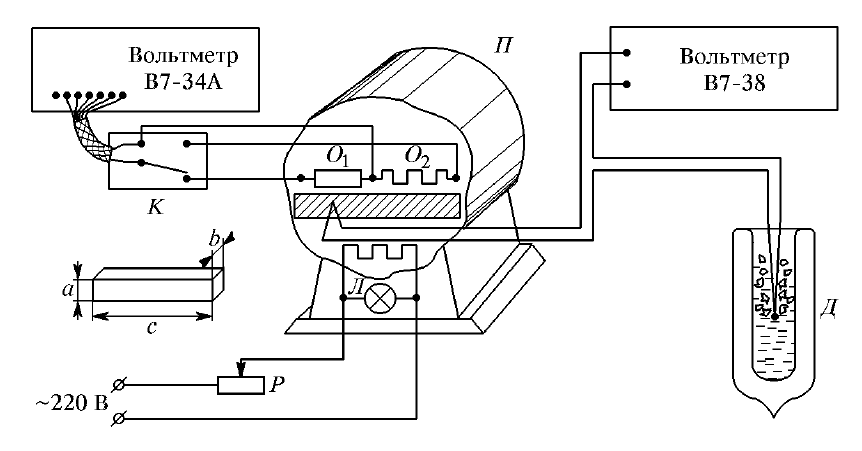
\includegraphics[width=0.5\textwidth]{scheme.png}
		\caption{Схема установки для измерения зависимости $\sigma(T)$}
		\label{pic:scheme}
	\end{figure} 
	
	Полупроводниковый образец имеет форму параллелепипеда, его параметры: $4.0 \times 4.0 \times 39$ (в мм). Медный образец - тонкая проволока длиной $l = 20$ м диаметра $d = 0.05$ мм.
	
	Удельная проводимость $\sigma$ связана с измеряемым сопротивлением $R$ следующей формулой: 
	
\begin{equation}\label{sigma}
	 \sigma = \frac{l}{RS} 
\end{equation}
	
	Здесь $l$ - длина образца, $S$ - его поперечное сечение.
	
	Температура образцов измеряется с помощью термопары, один спай которой расположен в печи, а другой - в сосуде Дьюара Д. 
	
	\section{Выполнение работы}
	
	В соответствии с графиком термопары, приложенным к установке, будем изменять значение напряжения на ней и устанавливать соответствующую температуру. Измерения начнем с $ T_0 = 26^\circ $
	
	Измерения зависимости сопротивлений меди $R_{Cu}$ и полупроводника $R_s$ от температуры $T$ приведены в таблице. Также рассчитаны $ \sigma $ по формуле \eqref{sigma} для полупроводника и меди, и значения $ 1/T$ и $ \ln \sigma, \ln \left( \dfrac{\sigma}{\sigma_0} \right) $, где $ \sigma_0 = \sigma (T_0) $. Построим графики зависимости $ \sigma (T) $ для полупроводника, а также график $ \ln \left( \dfrac{\sigma}{\sigma_0} \right) $ от $ 1/T $ для полупроводника. 
	
	 \begin{table}[h]
		\caption{Результаты измерений}
		\begin{center}
			\begin{tabular}{|c|c|c|c|c|c|c|c|c|c|}
				\hline
				$ №  $ & $ \eds $, мВ &  $ R_{пп} $, кОм & $ R_{Cu} $, кОм & $ T, ^\circ $ & $ \sigma_{пп} $, $ \dfrac{10^2}{Ом \x мм} $ & $ \sigma_{Cu} $, $  \dfrac{10^4}{Ом \x мм} $ & $ \dfrac{10^2}{T}, ^{\circ^{-1}} $ & $ \ln \sigma_{пп} $ & $ \ln  \dfrac{\sigma_{пп}}{\sigma_0} $\\
				\hline
			1 & -0.08 & 0.7703 & 0.091 & 26 & 0.3 & 6.69 & 3.85 & -5.8 & 0 \\
			2 & 0.12 & 0.604 & 0.0922 & 31 & 0.39 & 6.6 & 3.23 & -5.56 & 0.24 \\
			3 & 0.32 & 0.4775 & 0.0937 & 36 & 0.49 & 6.49 & 2.78 & -5.32 & 0.48 \\
			4 & 0.52 & 0.3805 & 0.0952 & 41 & 0.61 & 6.39 & 2.44 & -5.09 & 0.71 \\
			5 & 0.72 & 0.307 & 0.0969 & 46 & 0.76 & 6.28 & 2.17 & -4.88 & 0.92 \\
			6 & 0.92 & 0.2535 & 0.0984 & 51 & 0.92 & 6.18 & 1.96 & -4.69 & 1.11 \\
			7 & 1.12 & 0.2095 & 0.1 & 56 & 1.11 & 6.08 & 1.79 & -4.5 & 1.3 \\
			8 & 1.32 & 0.1736 & 0.1015 & 61 & 1.34 & 5.99 & 1.64 & -4.31 & 1.49 \\
			9 & 1.52 & 0.1456 & 0.1031 & 66 & 1.6 & 5.9 & 1.52 & -4.13 & 1.67 \\
			10 & 1.72 & 0.1215 & 0.1047 & 71 & 1.92 & 5.81 & 1.41 & -3.95 & 1.85 \\
			11 & 1.92 & 0.1038 & 0.1063 & 76 & 2.25 & 5.72 & 1.32 & -3.8 & 2 \\
			12 & 2.12 & 0.0882 & 0.1078 & 81 & 2.64 & 5.64 & 1.23 & -3.63 & 2.17 \\
			13 & 2.32 & 0.0757 & 0.1094 & 86 & 3.08 & 5.56 & 1.16 & -3.48 & 2.32 \\
			14 & 2.52 & 0.0651 & 0.111 & 91 & 3.58 & 5.48 & 1.1 & -3.33 & 2.47 \\
			15 & 2.72 & 0.0565 & 0.1125 & 96 & 4.13 & 5.41 & 1.04 & -3.19 & 2.61 \\
			16 & 2.92 & 0.0501 & 0.114 & 101 & 4.65 & 5.34 & 0.99 & -3.07 & 2.73 \\
				\hline
			\end{tabular}
		\end{center}
		\label{table_5}
	\end{table}
	
	
		\begin{figure}[h]
		\label{graf_pp}
		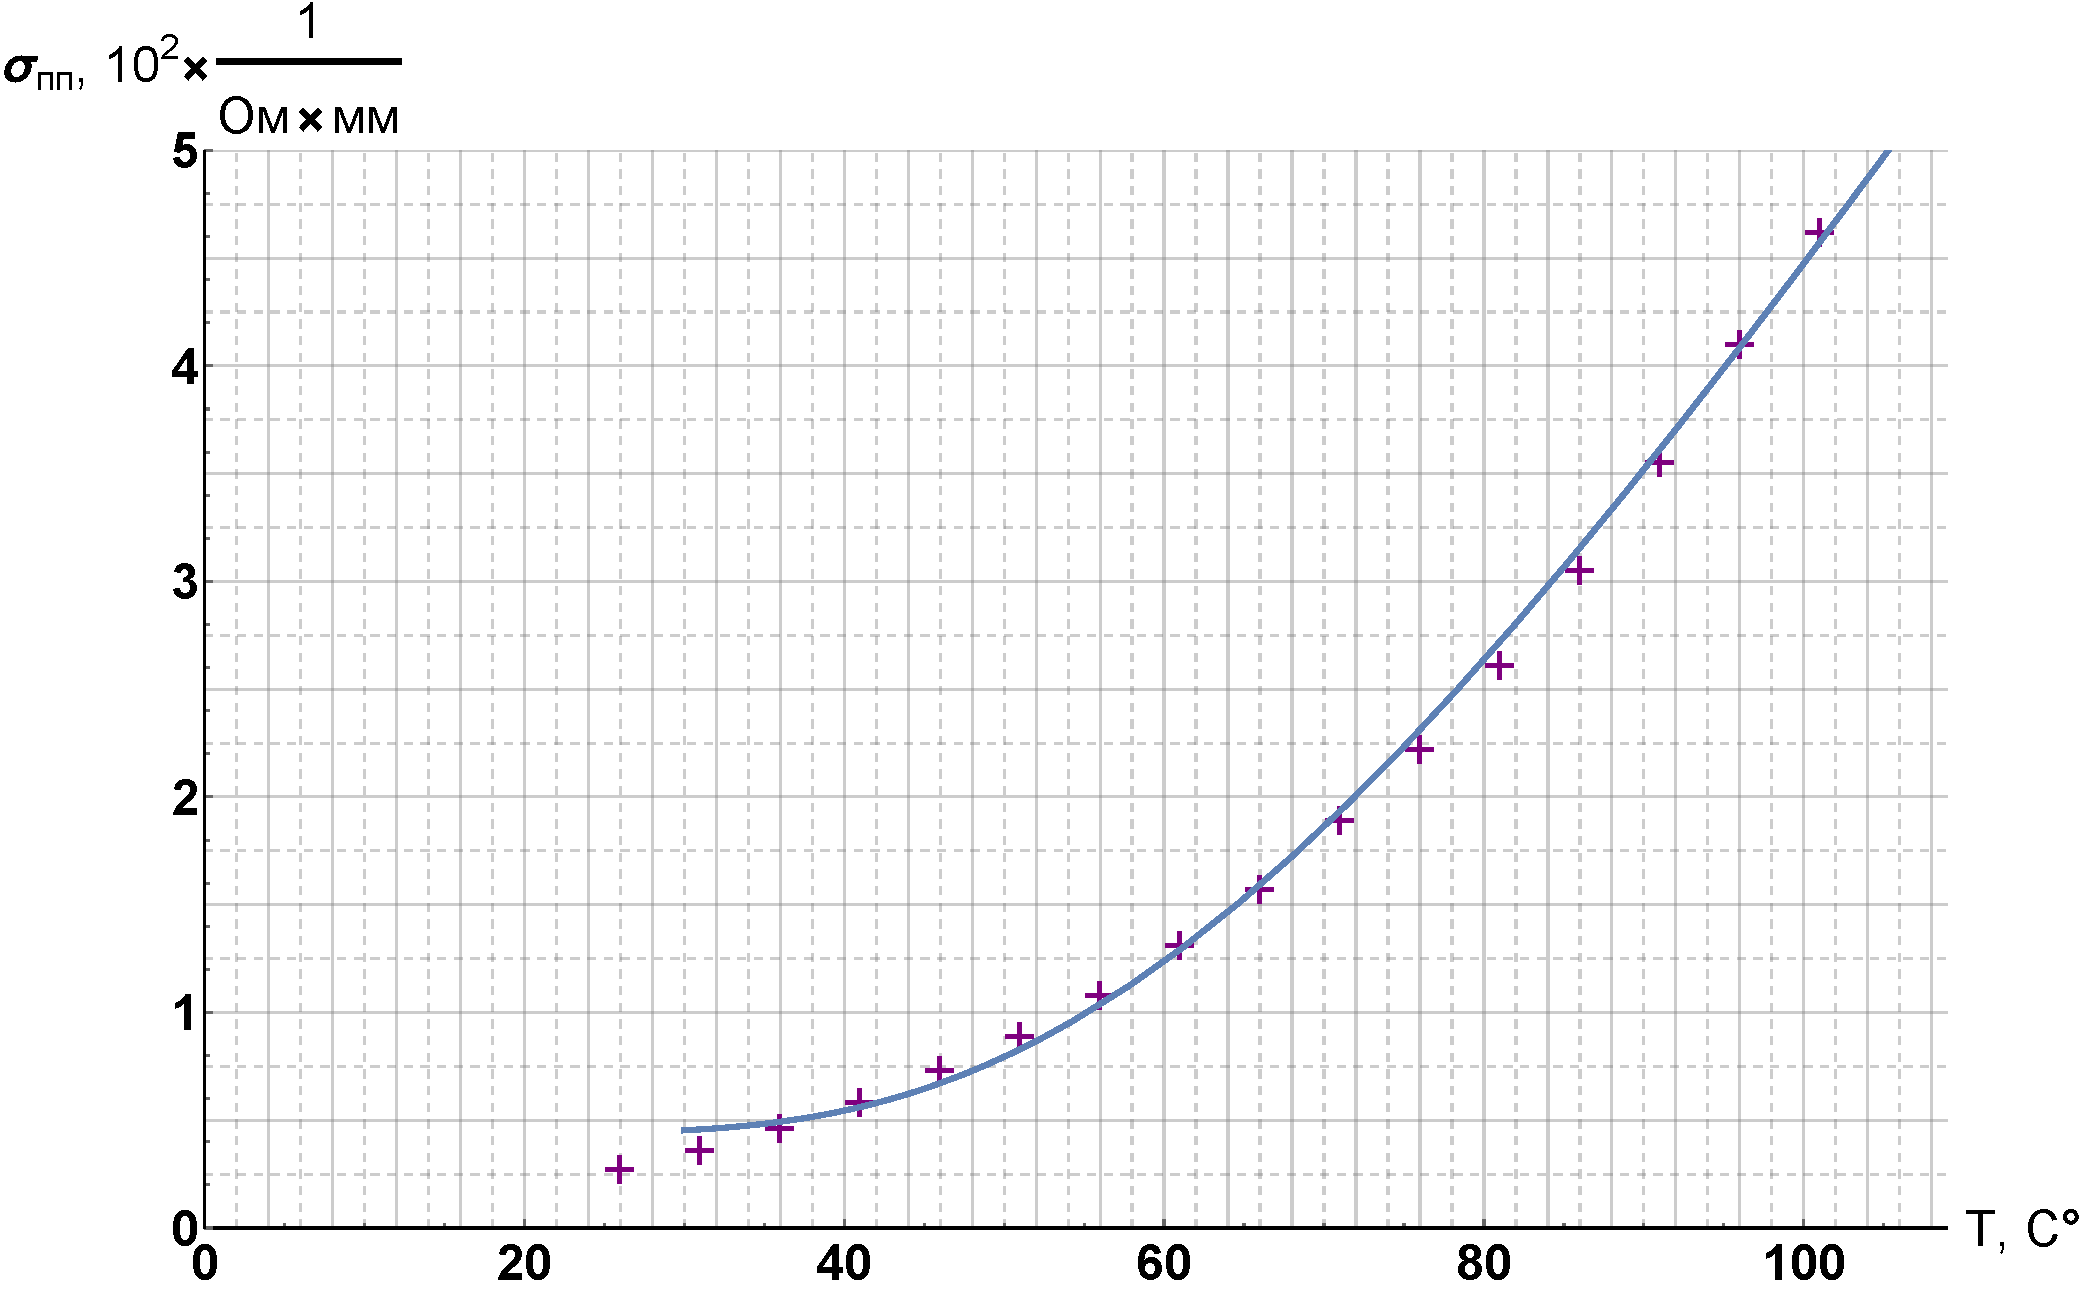
\includegraphics[scale=0.47]{pp.pdf}
		\caption{Зависимость $ \sigma(T) $ для полупроводника}
	\end{figure}
	
		\begin{figure}[h]
		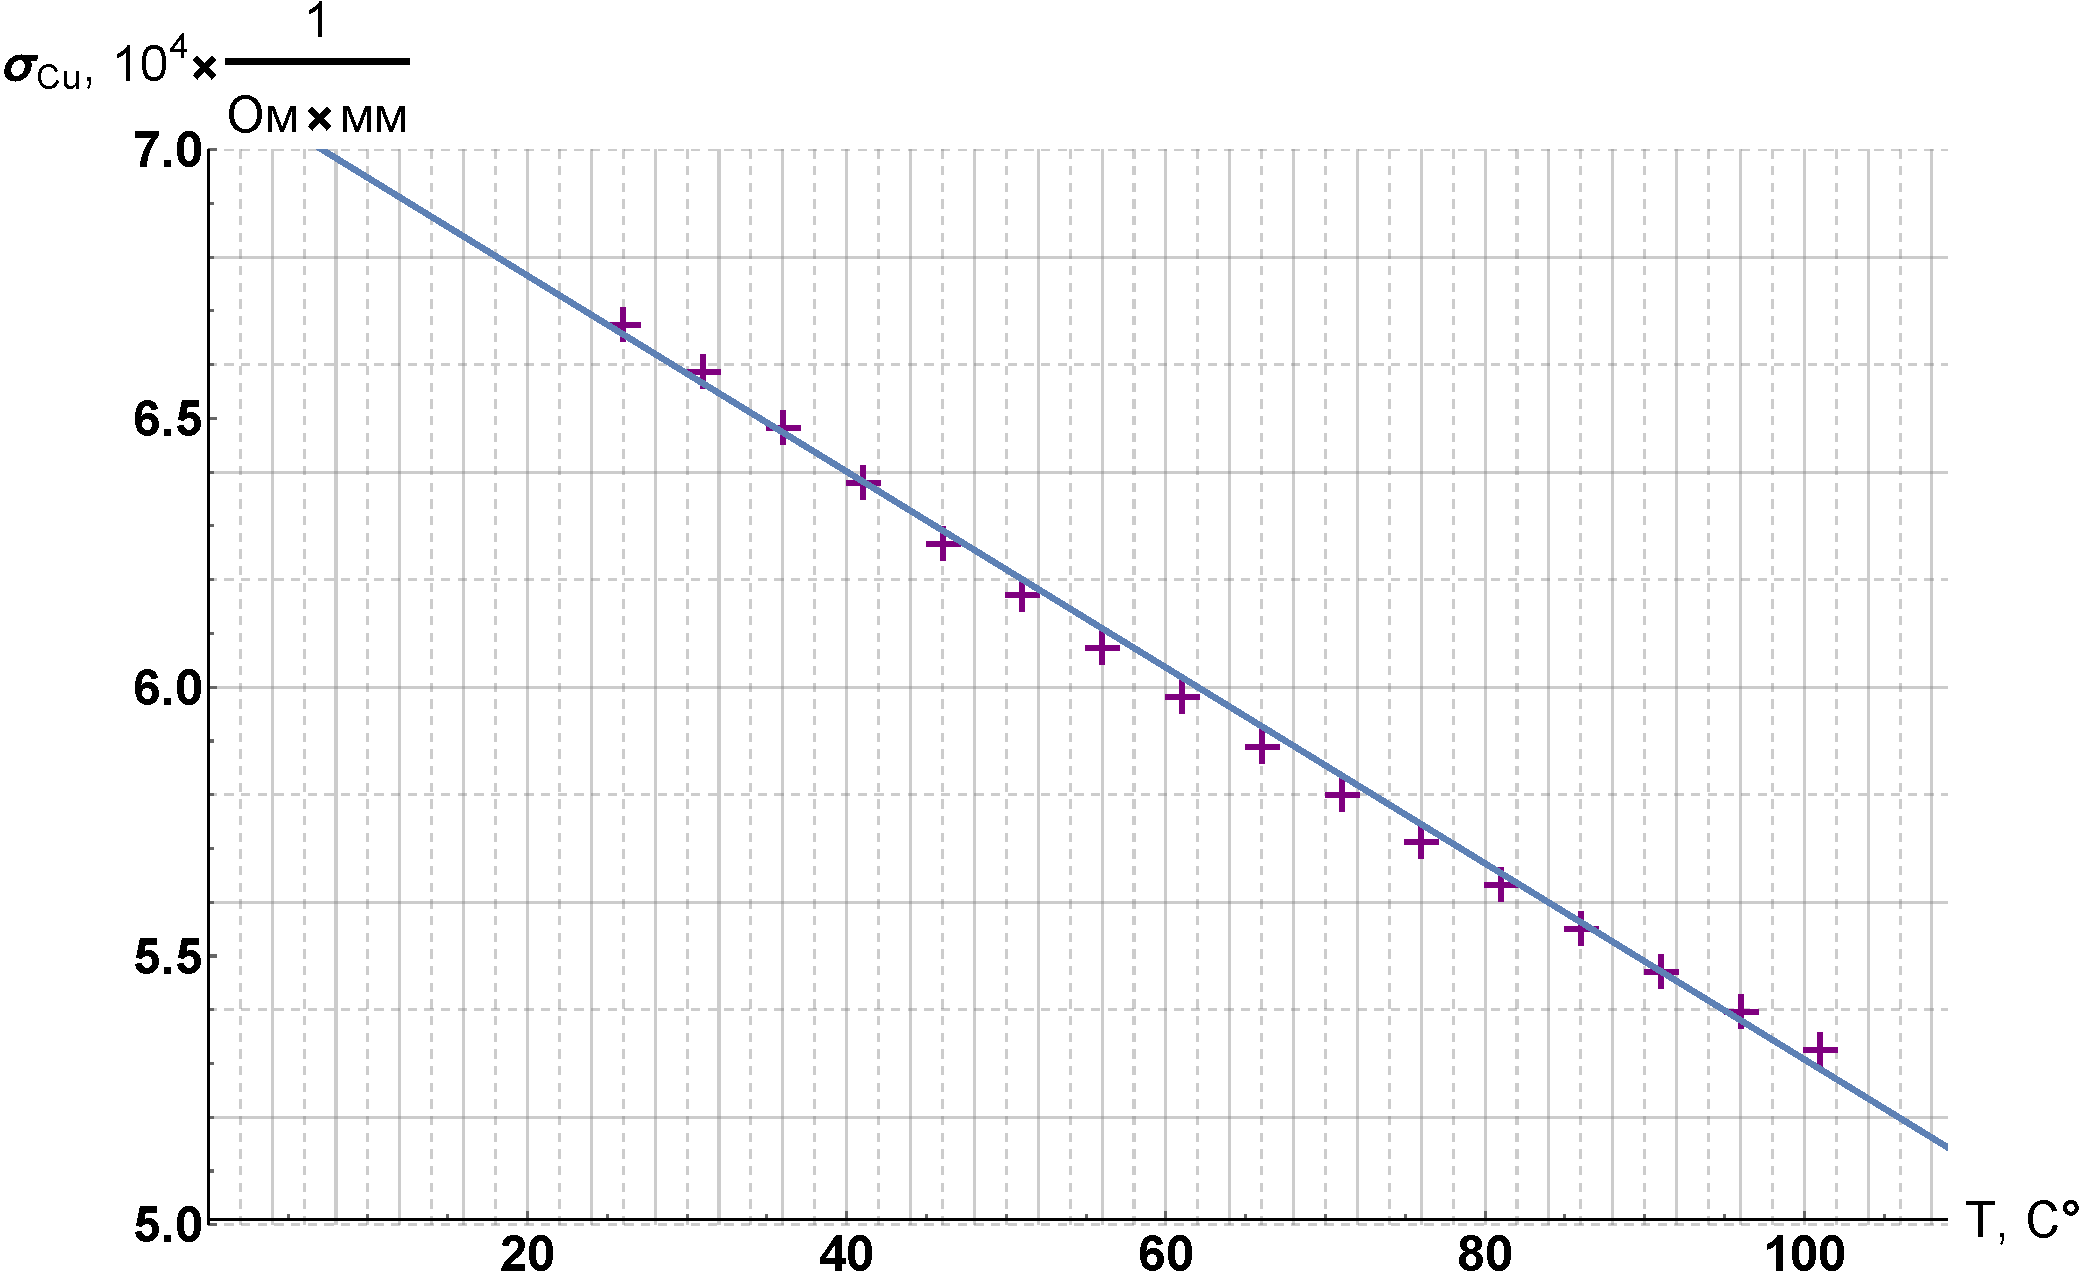
\includegraphics[scale=0.47]{cu.pdf}
		\caption{Зависимость $ \sigma(T) $ для меди}
				\label{graf_cu}
	\end{figure}

	\begin{figure}[h]
	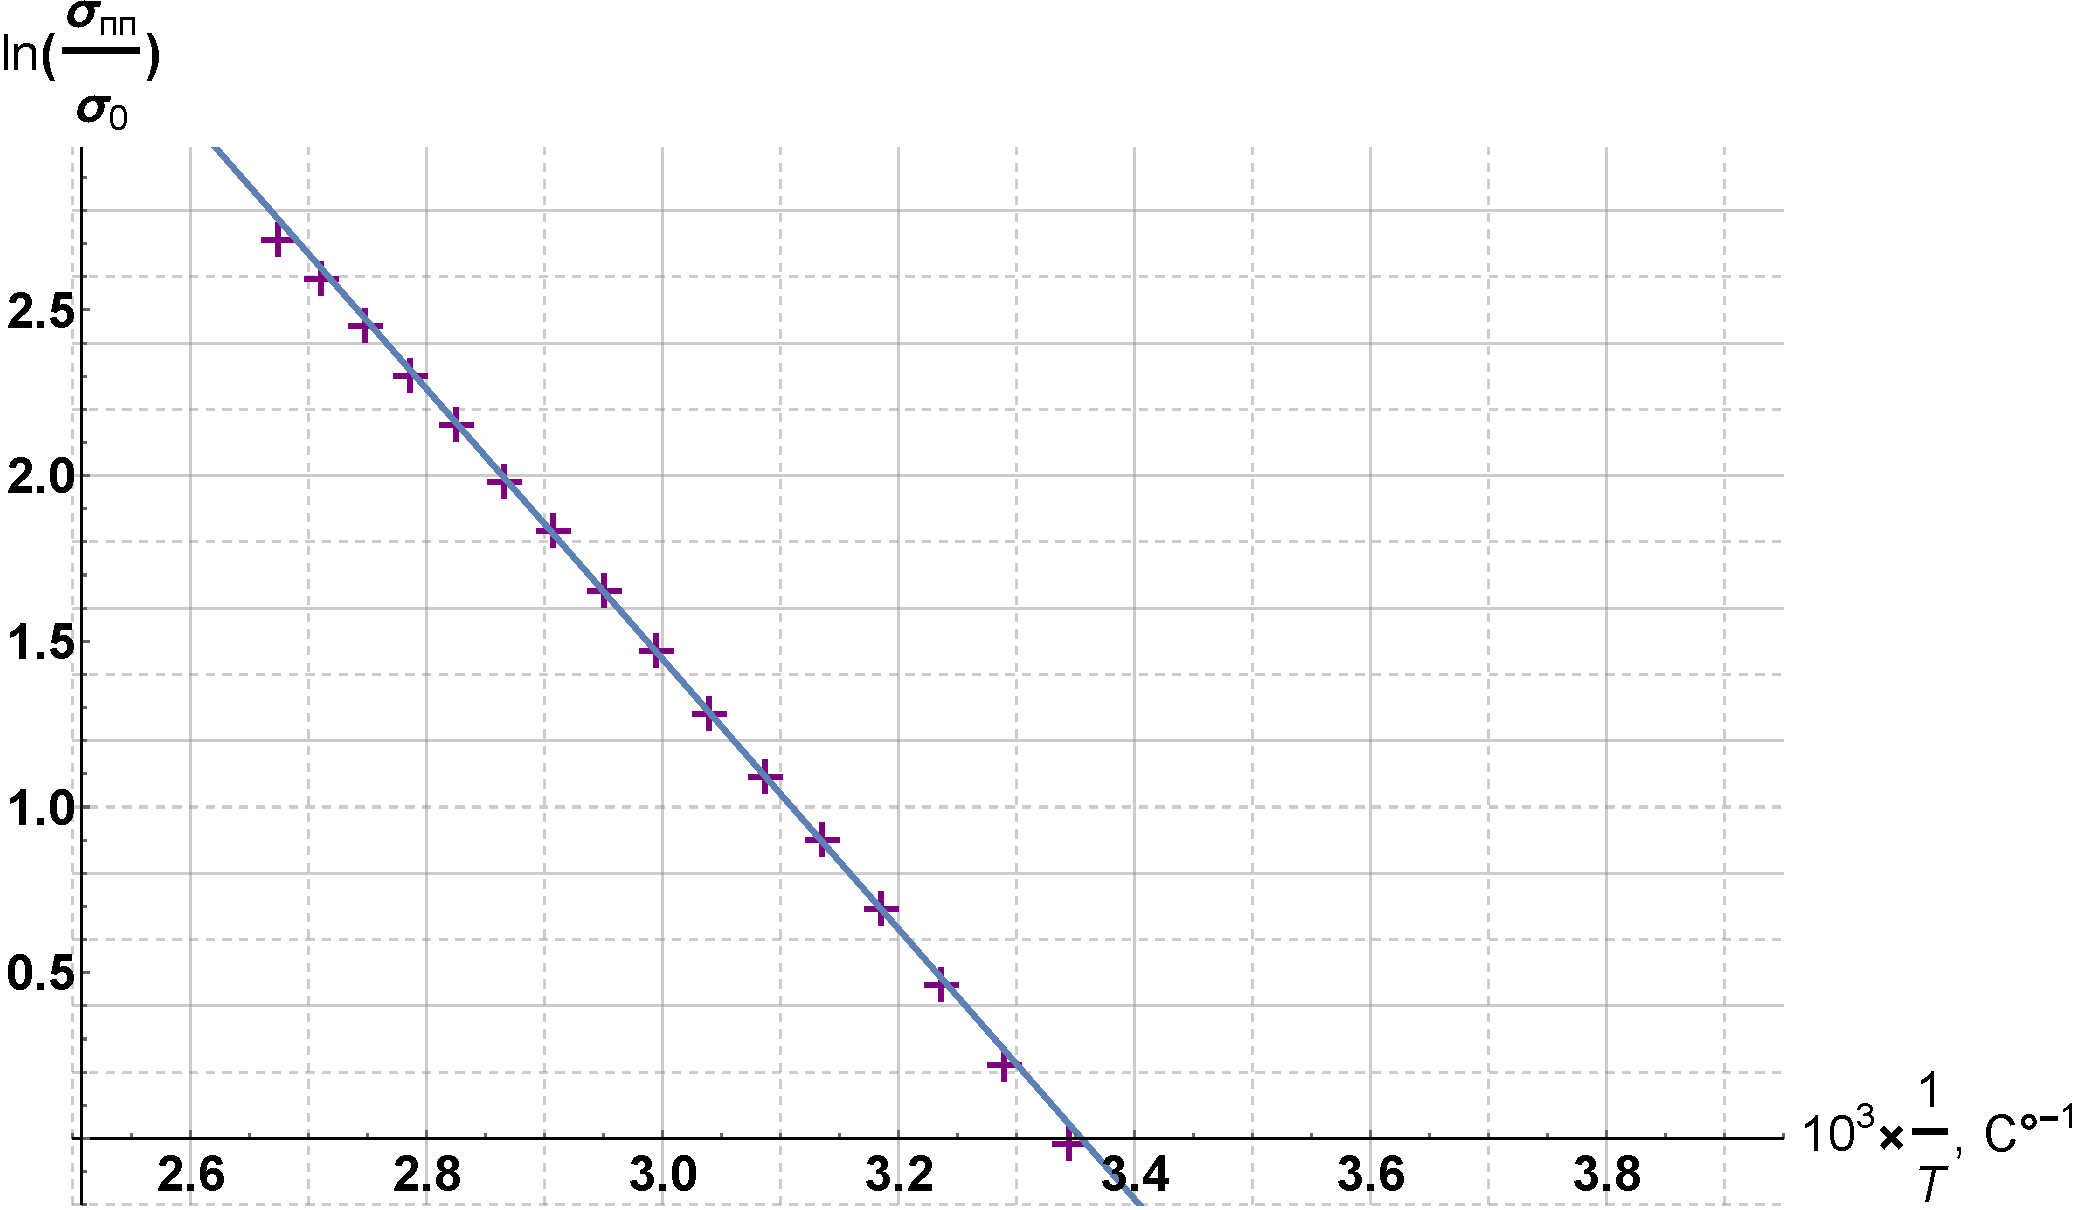
\includegraphics[scale=0.47]{ln.pdf}
	\caption{Зависимость $ \ln \left( \dfrac{\sigma}{\sigma_0} \right) $ от $ 1/T $ для полупроводника}
		\label{graf_ln}
\end{figure}

\begin{table}[H]
	\caption{Результаты фитов линейными ф-ми $ y = ax + b $}
	\begin{center}
		\begin{tabular}{|c|c|c|}
			\hline
			& \text{Estimate} & \text{Standard Error} \\
			\hline
			\multicolumn{3}{|c|}{Для графика рис. \ref{graf_cu}} \\
			\hline
			$ b $ & -0.94 & 0.45 \\
			$ a $ & 0.59 & 0.15 \\
			\hline 
			\multicolumn{3}{|c|}{Для графика рис. \ref{graf_ln}} \\
			\hline
			$ b $ & 13.667 & 0.085 \\
			$ a $ & -4.073 & 0.028 \\
			\hline
		\end{tabular} 
	\end{center}
	\label{}
\end{table}
	
	Из графика рис. \ref{graf_cu} получаем, что для $ \sigma_{Cu} = \dfrac{l}{R_{cu}S} = aT + b  \te $ %TODO
	
	Из графика зависимости  $ \ln \left( \dfrac{\sigma}{\sigma_0} \right) $ от $ 1/T $ для полупроводника мы получаем, 

	\begin{equation}\label{}
	\ln \left( \dfrac{\sigma}{\sigma_0} \right) = \dfrac{a'}{1000} \x \dfrac{1}{T} + b, \te  a' = -4073 \pm 28 \; К^{-1} = - \dfrac{\Delta}{2k} \te \Delta = 2 \x 4073 \x 8,6 \x 10^{-5} \approx 0,70 \pm 0,01 \; эВ
	\end{equation}
	
	Это значение очень близко к величине запрещенной зоны для \textbf{германия}: $ \Delta_{Ge} = 0,67 \;Эв $. 
	
	\section{Вывод }
	
	В работе мы проверили экспериментально проверили  зависимости проводимости металла и полупроводника от температуры --- они согласуются с теорией. Мы также определили температурный коэффициент сопротивления для меди 
	($ \alpha = $). %TODO
	Также мы получили ширину запрещённой зоны полупроводника, которая с хорошей точностью совпадает с табличной для германия.
	
	
\end{document}
